\documentclass[10pt,aspectratio=169]{beamer}
\usepackage{amsmath,amssymb,bm,booktabs,graphicx}
\usetheme{default}
\definecolor{HDSblue}{rgb}{0.2,0.2,0.7}
\setbeamertemplate{navigation symbols}{}
\setbeamertemplate{footline}{\hfill\usebeamerfont{page number in head/foot}\color{gray}\insertframenumber\,/\,\inserttotalframenumber\hspace{2mm}\vspace{2mm}}
\setbeamersize{text margin left=10mm,text margin right=8mm}
\setbeamercolor{frametitle}{fg=HDSblue}
\setbeamercolor{structure}{fg=HDSblue}
\setbeamerfont{frametitle}{size=\large}
\setbeamertemplate{itemize item}{\small$\blacktriangleright$}
\setlength{\parskip}{4pt}
\colorlet{blue}{HDSblue}
\title{How do model processes affect HBV simulation?}\subtitle{Calibration and process-switching experiments}\author{MMUQ Assignment 1 | Group presentation}\date{}
\begin{document}
% Speaker 1, approximately 4 minutes
\begin{frame}[plain]\titlepage\end{frame}
\begin{frame}{Research question and presentation roadmap}
\textcolor{HDSblue}{\textbf{Question:}} How does a calibrated HBV simulation respond when selected water pathways are switched off?
\begin{enumerate}\item Calibrate a baseline against observed discharge.\item Disable three groups of processes, keeping other parameters fixed.\item Compare hydrographs, storage and performance metrics.\item Discuss interpretation and limitations.\end{enumerate}
\medskip The focus is on \textbf{what the model does} when a process is removed.\end{frame}
\begin{frame}{Calibration: fitting HBV to the observed hydrograph}
\begin{columns}[T]\column{.51\textwidth}\begin{itemize}\item Supplied HBV001a and hourly inputs; catchment area 959 km$^2$.\item Nov 2010--Feb 2011: 2,880 hourly steps.\item 18 calibrated entries, including four initial storages.\item Differential Evolution (DE) searches the supplied parameter bounds.\end{itemize}
\column{.46\textwidth}\textcolor{HDSblue}{Objective:} minimise\[J(\theta)=1-\mathrm{NSE}=\frac{\sum_t(Q_{sim,t}-Q_{obs,t})^2}{\sum_t(Q_{obs,t}-\overline Q_{obs})^2}.\]
\small Large discharge errors receive greater weight because residuals are squared.\end{columns}\end{frame}
\begin{frame}{DE explores candidates and retains improvements}
\centering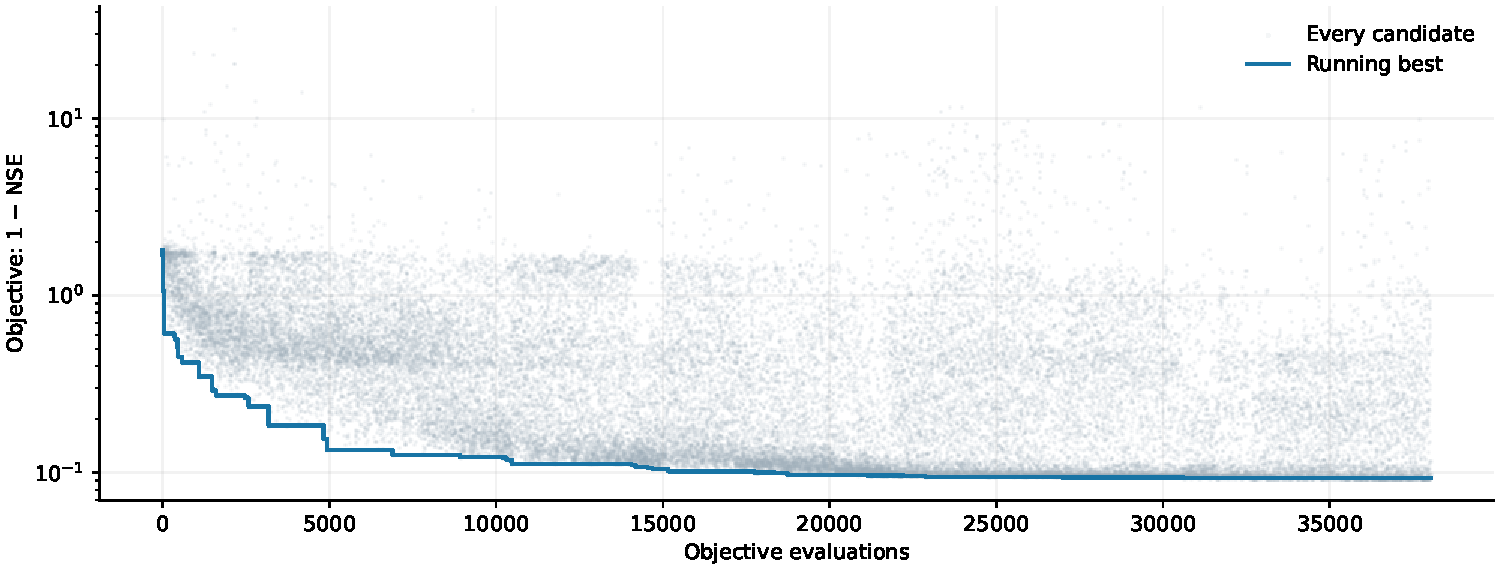
\includegraphics[width=.94\textwidth,height=.53\textheight,keepaspectratio]{figures/search_candidates.pdf}\\[-.2em]
\small Each candidate is a parameter vector: run HBV, calculate $J=1-\mathrm{NSE}$, then compare.\\
Grey: every attempted candidate. Blue: best value so far; \textbf{61 improvements} after the first.\\
Trials may be worse while the running best can only decrease or stay constant.\end{frame}
\begin{frame}{Why did the optimization stop?}
\centering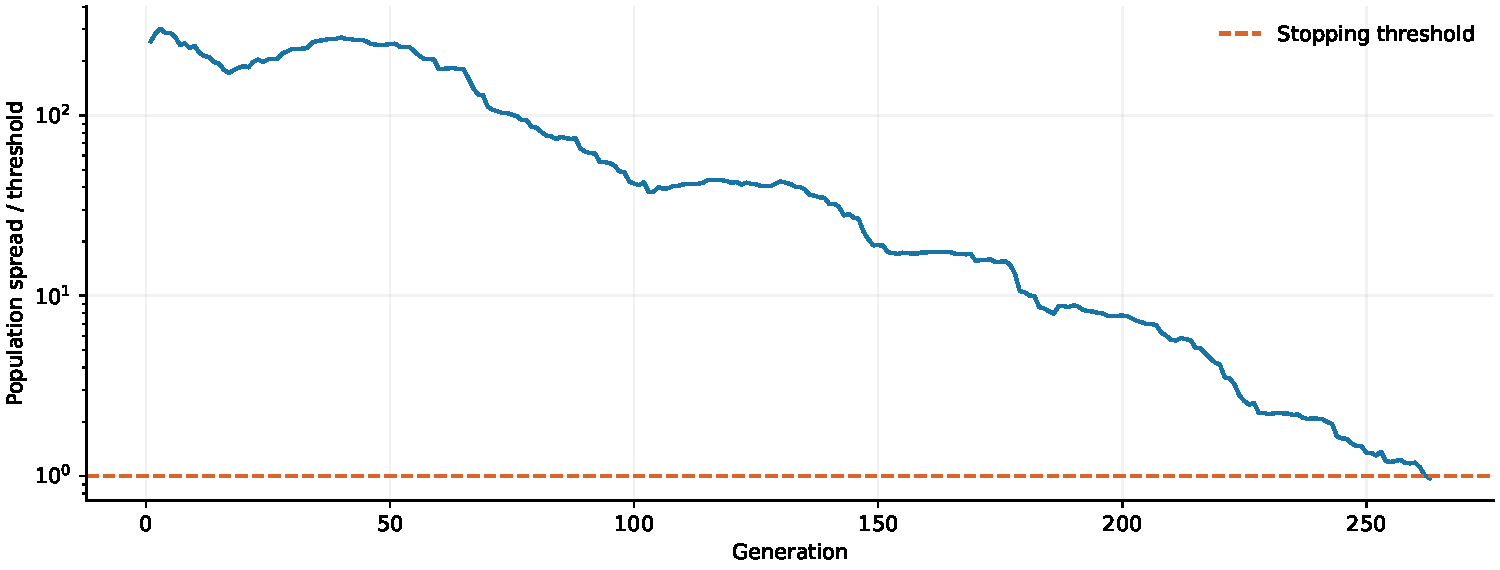
\includegraphics[width=.94\textwidth,height=.49\textheight,keepaspectratio]{figures/stopping.pdf}\\[-.2em]
\small Stop when $\operatorname{std}(J_{population})\leq 0.001\,|\operatorname{mean}(J_{population})|$.\\
At generation \textbf{263}: $9.10\times10^{-5}\leq9.32\times10^{-5}$; 38,016 evaluations.\\
Final $J=0.0930$ (NSE $=0.907$). Convergence \textbf{does not prove} a global optimum or unique parameters.\end{frame}
\begin{frame}{Baseline: good overall fit with an underestimated peak}
\centering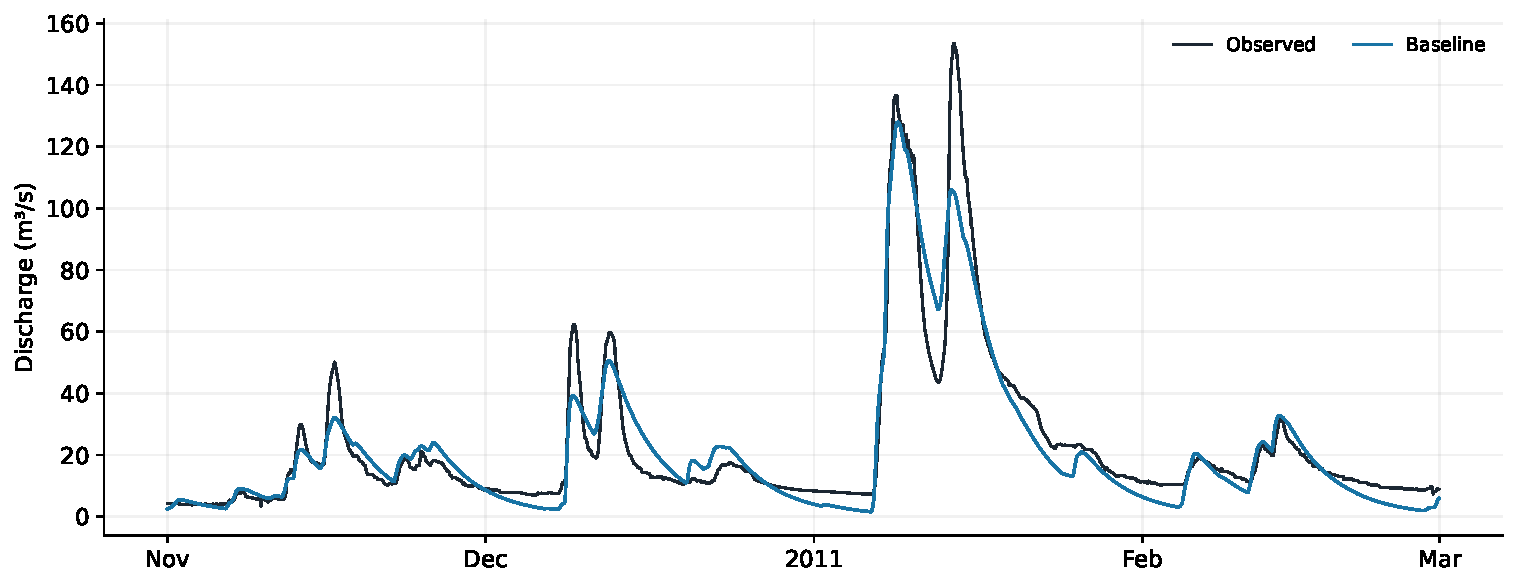
\includegraphics[width=.94\textwidth,height=.59\textheight,keepaspectratio]{figures/baseline.pdf}\\
\textbf{NSE 0.907} \quad | \quad \textbf{RMSE 7.86 m$^3$/s} \quad | \quad Volume bias $-5.0\%$\\
\small These are calibration-period metrics, not independent validation.\end{frame}
% Speaker 2, approximately 5 minutes
\begin{frame}{Baseline: zooming in on the largest observed event}
\centering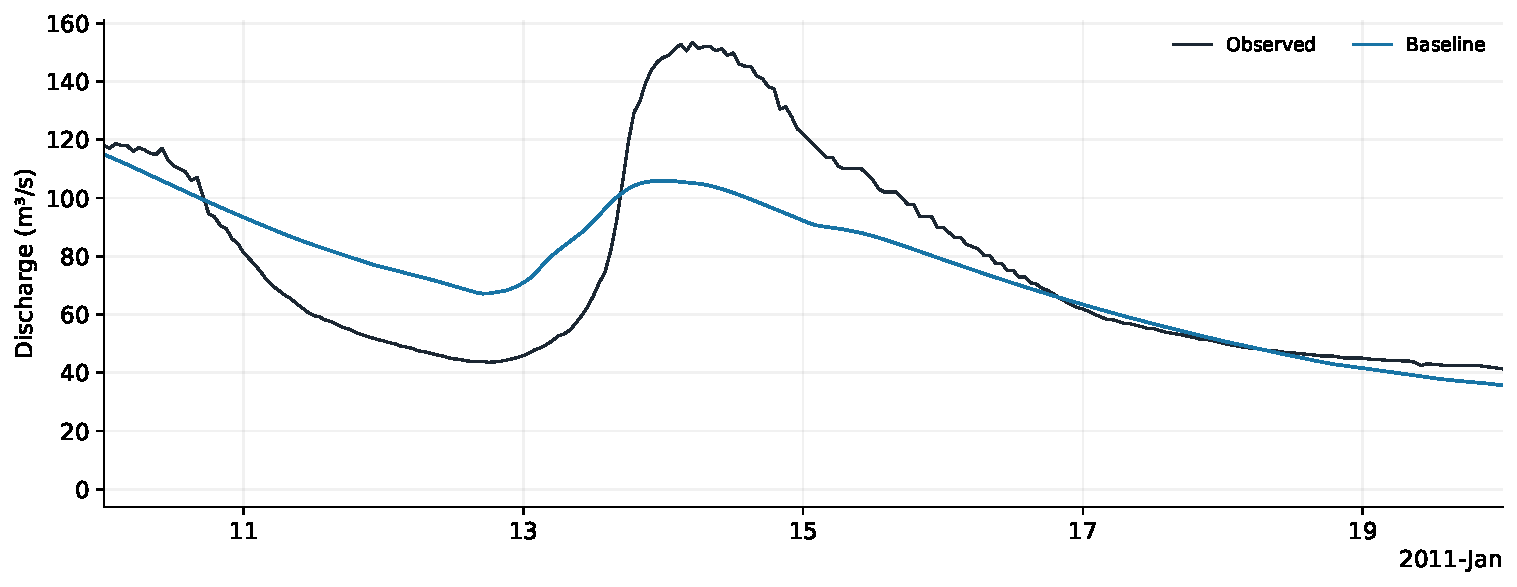
\includegraphics[width=.94\textwidth,height=.59\textheight,keepaspectratio]{figures/peak_zoom.pdf}\\
\small At the observed peak time: \textbf{153.5 observed vs 105.1 m$^3$/s simulated}.\\ This comparison is at the same timestamp; the simulated maximum can occur at another time.\end{frame}
\begin{frame}{Three process-switching experiments}
\small\begin{tabular}{p{.17\textwidth}p{.41\textwidth}p{.28\textwidth}}\toprule Experiment & Pathways disabled & Parameter(s) set to 0\\\midrule
Snowmelt & Rain-induced and air-induced melt & \texttt{snw\_pmf}, \texttt{snw\_amf}\\[.5em]
Channel outlets & Selected upper and lower reservoir outflows to channel & \texttt{urr\_ndr}, \texttt{lrr\_dre}\\[.5em]
Subsurface & Upper and lower subsurface exports & \texttt{urr\_uct}, \texttt{lrr\_lct}\\\bottomrule\end{tabular}
\medskip\begin{itemize}\item Change one group at a time; keep other parameters at baseline values.\item Same forcing, initial states and evaluation period; \textbf{no recalibration}.\end{itemize}\end{frame}
\begin{frame}{Experiment 1: turning off both snowmelt pathways}
\centering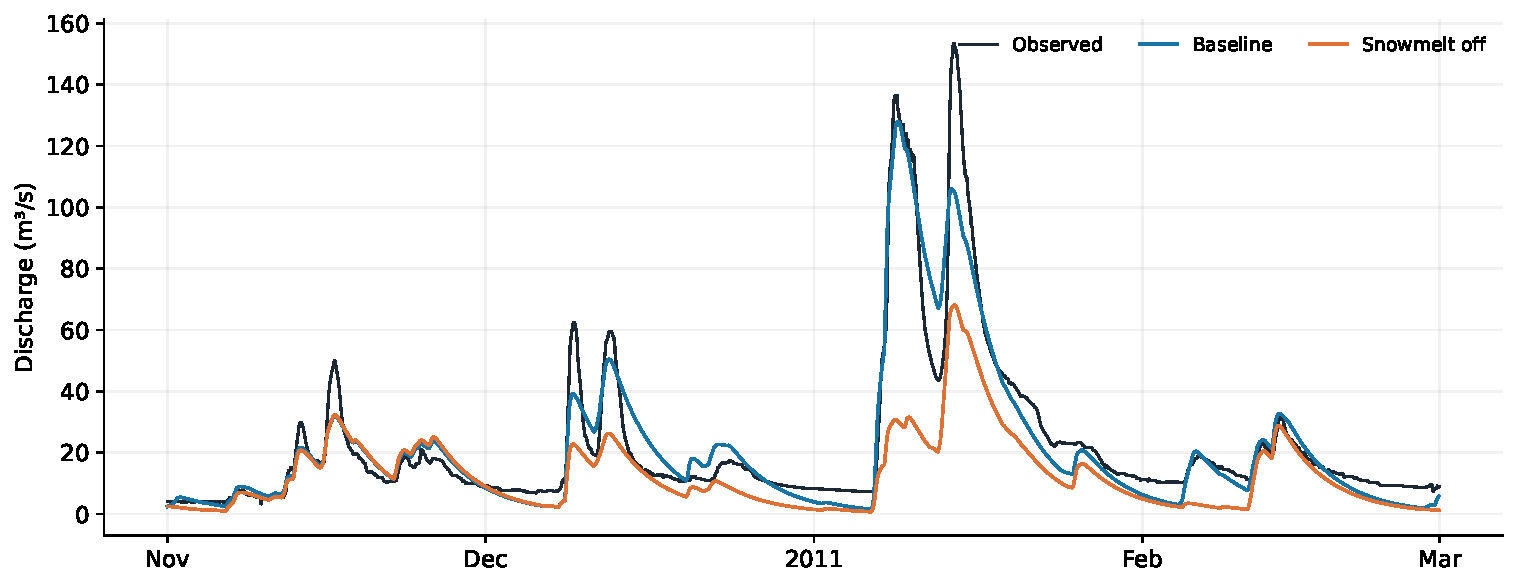
\includegraphics[width=.94\textwidth,height=.59\textheight,keepaspectratio]{figures/snow.pdf}\\
\small NSE \textbf{0.907 $\rightarrow$ 0.414}; volume bias $-5.0\%\rightarrow-43.0\%$.\\ Several events are reduced when snow cannot melt through these paths.\end{frame}
\begin{frame}{Snowmelt: what happens around the January peak?}
\centering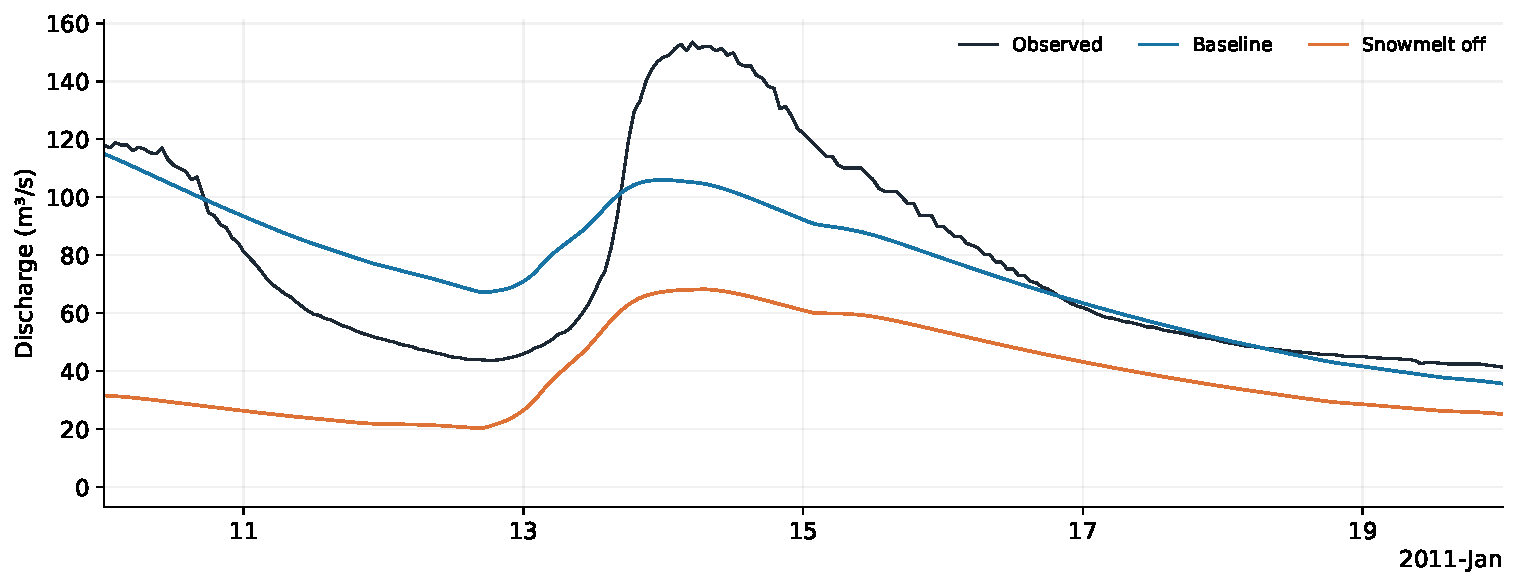
\includegraphics[width=.94\textwidth,height=.59\textheight,keepaspectratio]{figures/snow_zoom.pdf}\\
\small At the observed peak time: baseline 105.1; melt off 68.1; observed 153.5 m$^3$/s.\\ The change is a model response under the fixed baseline parameters.\end{frame}
\begin{frame}{Snowmelt: water remains in snow storage}
\centering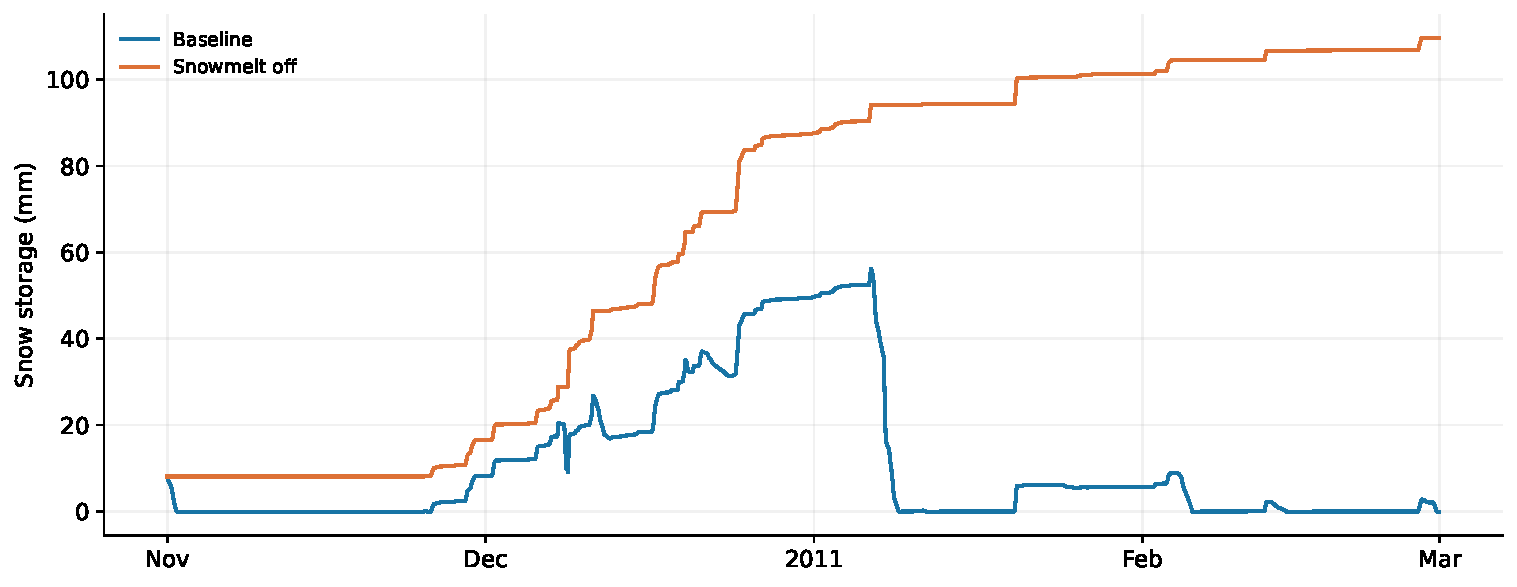
\includegraphics[width=.94\textwidth,height=.59\textheight,keepaspectratio]{figures/snow_storage.pdf}\\
\small Snow can still accumulate, but the two melt terms are zero.\\ End-of-period snow: \textbf{109.5 mm}, compared with 0.0 mm for the baseline.\end{frame}
% Speaker 3, approximately 5 minutes
\begin{frame}{Experiment 2: selected channel outlets off}
\centering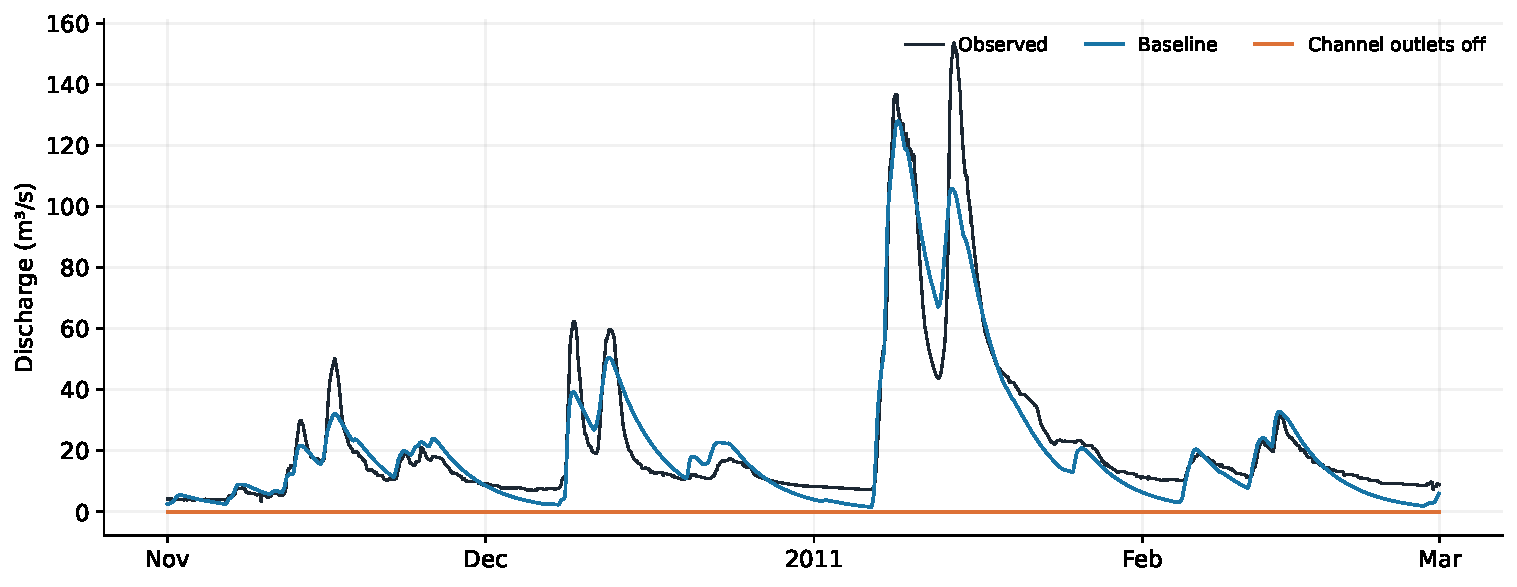
\includegraphics[width=.94\textwidth,height=.59\textheight,keepaspectratio]{figures/outlets.pdf}\\
\small Simulated channel discharge is zero throughout this run; NSE $=-0.754$.\\ The separate upper threshold outlet remains enabled, but does not activate here.\end{frame}
\begin{frame}{Channel outlets: the lower reservoir fills}
\centering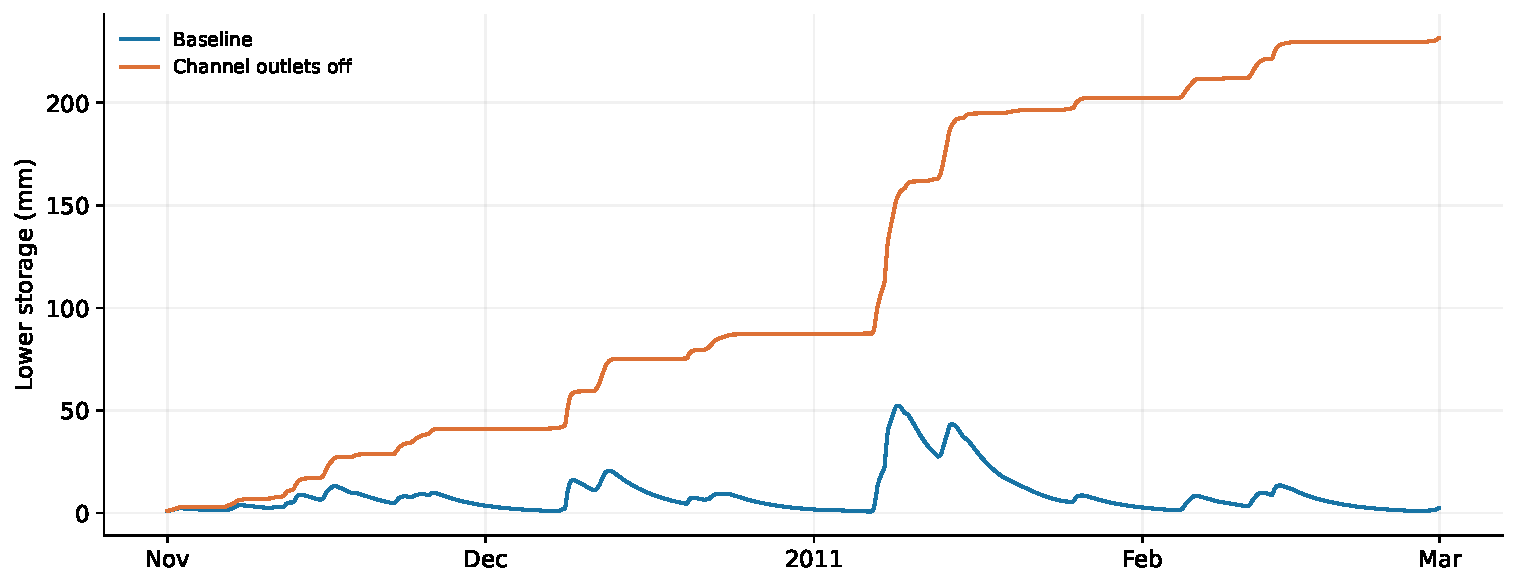
\includegraphics[width=.94\textwidth,height=.59\textheight,keepaspectratio]{figures/lower_storage.pdf}\\
\small Final lower storage: \textbf{231.5 mm}, versus 2.4 mm in the baseline.\\ Water remains in the model rather than exiting through the disabled paths.\end{frame}
\begin{frame}{Experiment 3: subsurface exports off}
\centering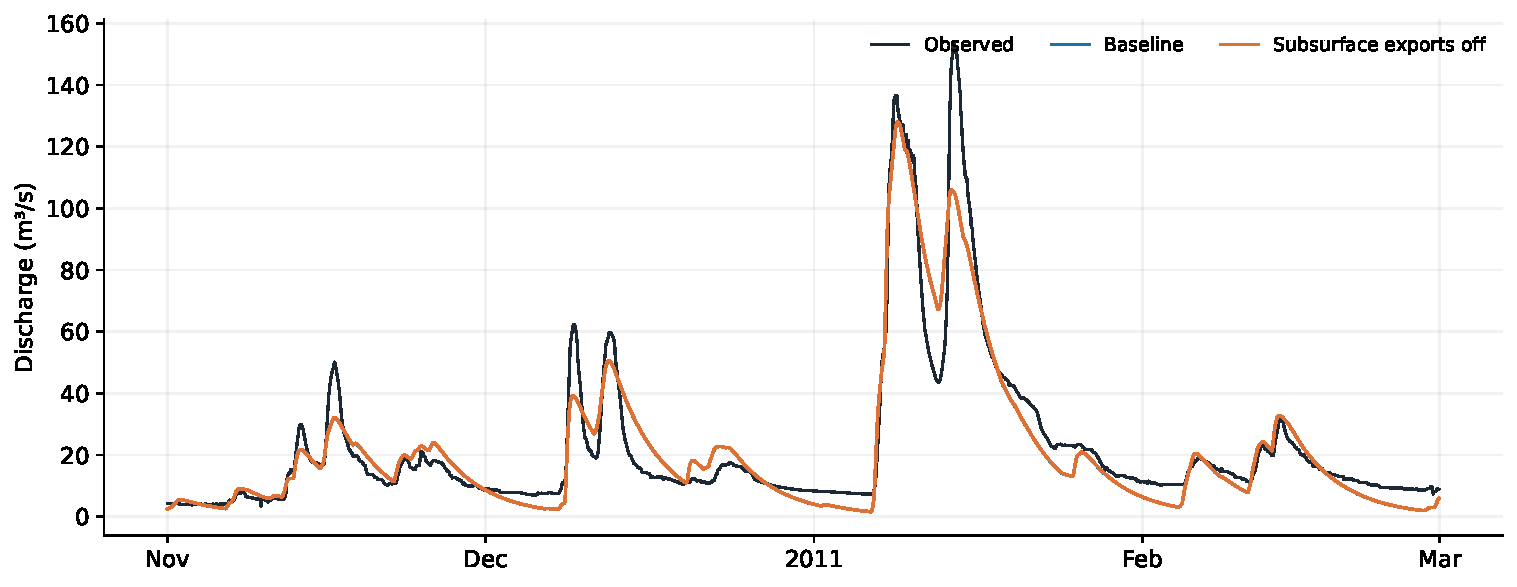
\includegraphics[width=.94\textwidth,height=.59\textheight,keepaspectratio]{figures/subsurface.pdf}\\
\small Curves nearly overlap: NSE 0.906972 $\rightarrow$ 0.906997.\\ The baseline export coefficients are already close to zero.\end{frame}
\begin{frame}{Subsurface exports: reveal the small difference}
\centering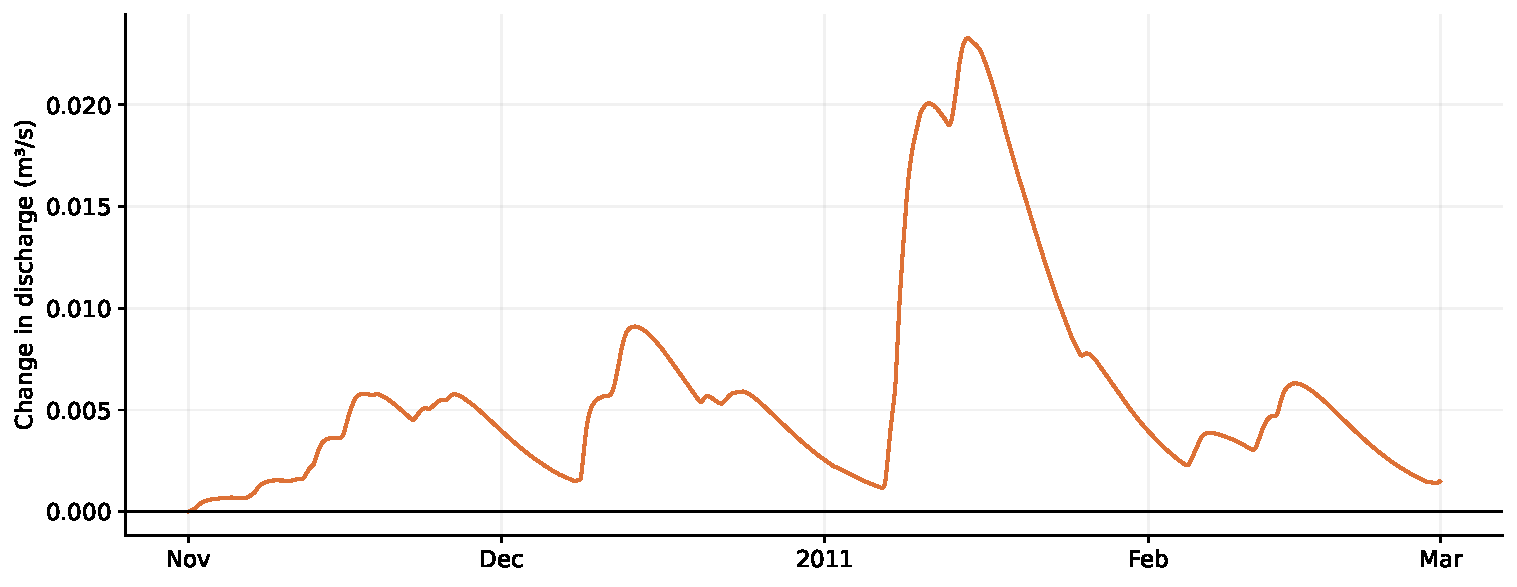
\includegraphics[width=.94\textwidth,height=.59\textheight,keepaspectratio]{figures/subsurface_difference.pdf}\\
\small Maximum absolute change in discharge is approximately \textbf{0.0233 m$^3$/s}.\\ Subsurface exports affect stored water and can influence channel flow indirectly.\end{frame}
% Speaker 4, approximately 5 minutes
\begin{frame}{Comparing the three experiments}
\begin{center}\small\begin{tabular}{lrrr}\toprule Case & NSE & RMSE (m$^3$/s) & Volume bias\\\midrule
Baseline & 0.907 & 7.86 & $-5.0\%$\\ Snowmelt off & 0.414 & 19.73 & $-43.0\%$\\ Selected channel outlets off & $-0.754$ & 34.12 & $-100.0\%$\\ Subsurface exports off & 0.907 & 7.86 & $-5.0\%$\\\bottomrule\end{tabular}\end{center}
\medskip\begin{itemize}\item The first two interventions have large effects on discharge and storage.\item The third has little effect under this calibrated parameter set.\item NSE can be negative; zero corresponds to predicting the observed mean.\end{itemize}\end{frame}
\begin{frame}{Interpretation: what do these experiments tell us?}
\begin{itemize}\item \textbf{Snowmelt:} freezing melt terms holds water in snow and changes the timing and volume of runoff.\item \textbf{Channel outlets:} disabling two outflows disrupts the discharge pathway and increases storage.\item \textbf{Subsurface:} a near-zero baseline coefficient leaves little immediate effect to remove.\end{itemize}
\medskip These are model-specific responses, not direct measurements of process contribution in the catchment.\end{frame}
\begin{frame}{Limitations and next steps}
\begin{itemize}\item No recalibration after switching: parameter compensation has not been tested.\item The full record is used for calibration, with no warm-up or held-out validation.\item NSE emphasizes squared errors; also assess peak timing, volume and low flows.\item One DE run reached its stopping criterion, which does not establish a unique or global optimum.\end{itemize}
\medskip\textcolor{HDSblue}{Next:} Recalibrate selected simplified models and evaluate them on independent data.\end{frame}
\begin{frame}{Conclusions and questions}
\begin{enumerate}\item Baseline NSE is 0.907, but the largest observed peak is underestimated at its timestamp.\item Turning off melt or selected channel outlets substantially changes discharge and storage.\item Turning off subsurface exports barely changes this particular baseline simulation.\end{enumerate}
\medskip\textcolor{HDSblue}{Discussion:} Which process experiments should we recalibrate? What validation period and performance metrics should we use?\end{frame}
\end{document}